%!TEX root = ../paper.tex

\subsubsection{Data Recipient}
Across all scenarios, 42\% of participants stated that they would be ``very upset'' if their data was shared with only the app's servers, whereas the VURs for friends (70\%), work contacts (75\%), and the public (72\%) were much higher (Table \ref{recipient-vur}). A chi-square test indicated that these differences were statistically significant (Table \ref{recipient-chi}). However, these effect sizes were small: the largest effect was between work contacts and an app's server ($\phi=0.11$); while the VUR for sharing with work contacts was significantly higher than sharing with friends, the effect size was negligible ($\phi=0.004$). 

We note that this chi-square test violates the assumption of independent observations, since participants responded to multiple scenarios. But based on the randomization of treatments and large sample size, we do not believe that this significantly impacted our results. Similarly, we are unaware of a more appropriate test, given our data format; Cochran's Q requires binary outcomes (i.e., participants would have had to answer only one question for each data recipient, preventing us from adequately controlling for data type) and a repeated measures ANOVA requires normality (our data was not normally distributed). Nonetheless, we repeated our analysis using only one randomly-selected data point per participant and found that our selected test was robust to this violation. Participants were significantly more concerned about having their data seen by humans ({\it vis-{\`a}-vis} app servers), though differences between specific human groups (between the public, friends, and work contacts) were not significant. 

{\color {red} We do not claim that there is no distinction between the friends, public, and work contact recipients, because people have been shown to behave differently, especially in the social arena (cite studies here). People are more comfortable sharing certain data types with certain recipients (refer to the table of all questions with ranks by each recipient here). There are other data types which are universally concerning, and universally unconcerning, and the magnitude of the sentiment varies by recipient. As you can see in Table (J still needs to do this table), the VUR rate for each recipient is negatively correlated with the standard deviation of the answers.  Additionally, we see that there is greater distinction between sharing people and the app server--people are comfortable sharing data they would feel uncomfortable sharing with at human recipient, and the magnitude of concerns is might more significant compared to the other recipients.}

\begin{table}[t]
\begin{center}
\small
\begin{tabular}{| r | l | r | l |c |}
\hline
Rank & Recipient & VUR & sigma & Distribution \\
\hline
1 & Work Contacts & 75.16\% & 0.94 & 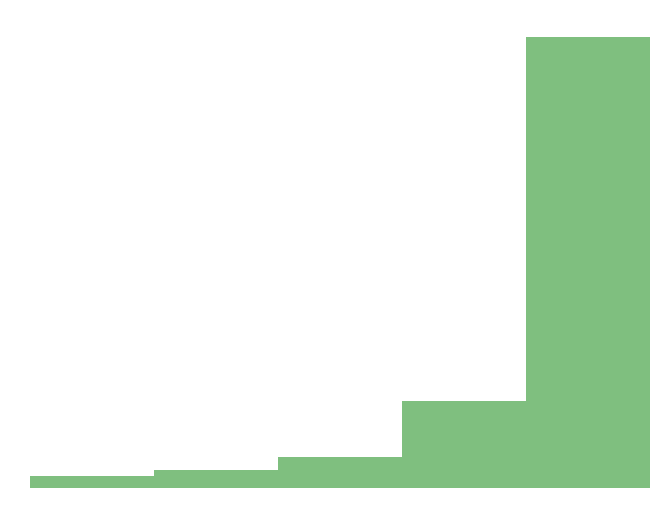
\includegraphics[width = 2cm, height = 0.5cm]{tex-inputs/recipient4/recipient_work} \\
2 & Public & 72.41\% & 0.98 & 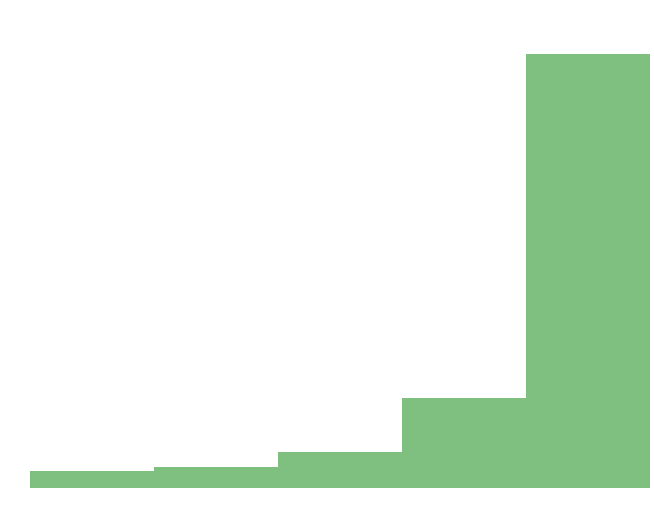
\includegraphics[width = 2cm, height = 0.5cm]{tex-inputs/recipient4/recipient_pub}  \\
3 & Friends & 69.47\% & 1.02 & 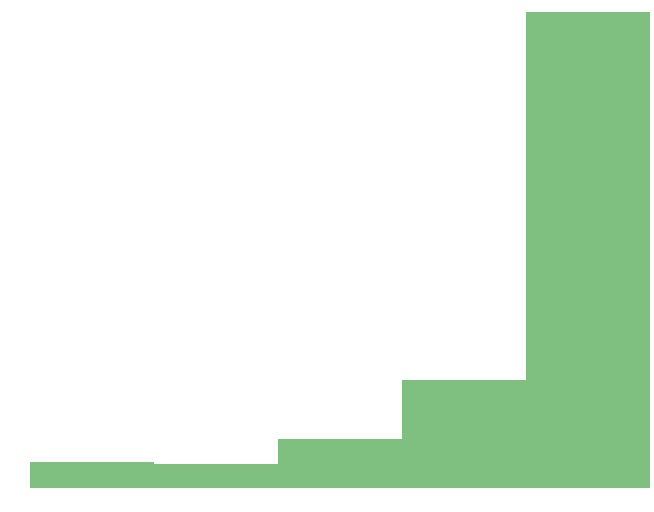
\includegraphics[width = 2cm, height = 0.5cm]{tex-inputs/recipient4/recipient_friends}\\
4 & App's Server & 42.28\% & 1.15 & 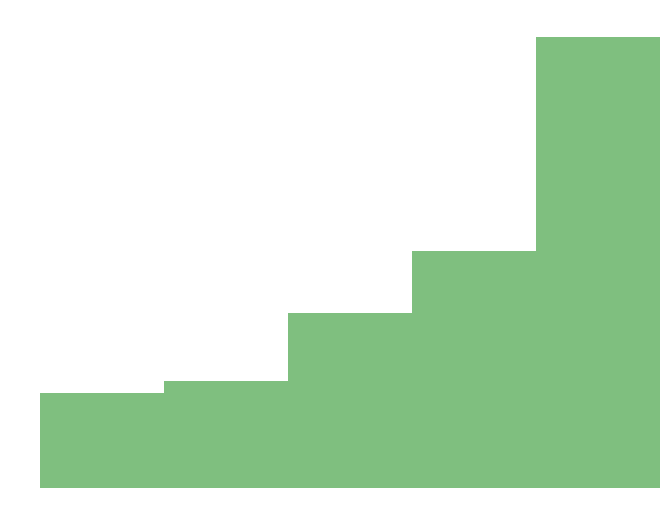
\includegraphics[width = 2cm, height = 0.5cm]{tex-inputs/recipient4/recipient_app}\\
\hline
\end{tabular}
\caption{The overall upset rate for all recipients.}
\label{recipient-vur}
\end{center}
\end{table}

\begin{table}[t]
\begin{center}
\begin{tabular}{|l|r|r|r|r|}
\hline
Recipients	& $\chi^2$ & p-value 	& n & $\phi$ \\
\hline
Work-App	& 565.910 & <0.0001 & 5,083 & 0.111\\
Public-App	& 481.776 & <0.0001 & 5,1988& 0.093\\
Friends-App & 381.653 & <0.0001 & 5,096 & 0.075\\
Friends-Work & 20.39 & <0.0001 & 5,037 & 0.004\\
Friends-Public & 5.41 & <0.0200 & 5,142 & 0.001\\
Work-Public&  5.00 & <0.0253 & 5,129	& 0.001\\
\hline
\end{tabular}
\caption{Results of a chi-square test to examine VUR based on data recipient, across all data points.}
\label{recipient-chi}
\end{center}
\end{table}

{\color {red} TODO: table of top and bottom 10 data types by recipient; refer to appendix; shoutout to when you were lying nervous or stressed work}
